\documentclass[12pt, a4paper]{report}

\usepackage[utf8]{inputenc}
\usepackage{graphicx}
\usepackage{listings}
\usepackage{mathtools}
\usepackage{amsmath}
\usepackage{amssymb}
\usepackage{subcaption}
\usepackage{geometry}
\usepackage{color}
\usepackage{url}

\usepackage{pgf,tikz}\usepackage{mathrsfs}\usetikzlibrary{arrows}

\usepackage[]{geometry}

\usepackage{hyperref}
\hypersetup{
    colorlinks,
    citecolor=black,
    filecolor=black,
    linkcolor=black,
    urlcolor=black
  }  

\renewcommand{\contentsname}{Contenidos}
\renewcommand{\chaptername}{Capítulo}
\renewcommand{\figurename}{Figura}


\title{Treball de Recerca:\\Teoría e implementación de un motor gráfico}
\date{Curso 2017/2018}
\author{Alumno: Joel Pérez\\Profesor: José Ramírez\\Departamento de Matemáticas}


\begin{document}
\lstset{language=C, basicstyle=\ttfamily}
\pagenumbering{gobble}

\maketitle


\newpage

\pagenumbering {arabic}

\begin{abstract}
  En este Treball de Recerca he intentado demostrar cómo funcionan las principales librerías gráficas comerciales y poder entender los diversos cálculos que se efectúan en la ejecución de una aplicación gráfica 3D. Para esto he programado una librería gráfica relativamente simple y la he usado en un motor gráfico que también he programado.
\end{abstract}

\renewcommand{\abstractname}{Agradecimientos}
\begin{abstract}
  Me gustaría dar las gracias a todos los profesores que he tenido a lo largo de mi vida, en especial a José Ramírez por ser un brillante tutor que además ha invertido mucho de su tiempo libre en ayudarme.

  También me gustaría agradecer a mis familiares y mis amigos por soportarme, en especial a mi gran amigo Ori, por introducirme a la programación orientada a gráficos y darme la idea para este TdR.

\end{abstract}

\tableofcontents

%% Introducción 
\chapter{Introducción}
\section{Resumen}
Una revolución industrial consiste en la llegada de nuevas máquinas y métodos que permiten optimizar los procesos de producción. La industria del software está pasando actualmente por una de estas revoluciones, dónde están surgiendo multitud de herramientas para agilizar la producción. Estas herramientas oscilan desde librerías para funciones matemáticas simples, pasando por editores de texto inteligentes que van acompañados por un compilador y depurador (\textit{IDE}s) e incluso llegan a motores gráficos comerciales disponibles a cualquier programador con una habilidad intermedia, permitiendo saltar uno de los pasos más laboriosos del proceso de creación de videojuegos.

La llegada de esta ola ha sido bastante polémica y ha dividido a las comunidades. Por una parte no se puede negar la importancia de tener herramientas más potentes. Pero por la otra parte hay muchos que piensan que esto ha llevado a la gente a no preocuparse por algunas cuestiones sólo porque lo ven como una cosa del pasado, un problema menor que ya está solucionado por la herramienta que usan. Estos problemas terminan por acumularse y pueden desencadenar en problemas mayores si no se intentan solventar desde la raíz.

Mi opinión siempre ha sido la de permanecer escéptico a los programas que pretenden tener un uso generalizado, y siempre he creído que cada herramienta es para una situación concreta, y no se puede intentar usar el mismo método y herramientas para todo.

\newpage
\section{Objetivos}
Según la prioridad asignada he separado los objetivos en dos categorías. Es importante recordar que \textbf{no es un objetivo} obtener un producto de una complejidad y rendimiento similar a librerías y motores gráficos comerciales.
\subsection{Objetivos principales}
\begin{itemize}
\item Investigar la factibilidad de desarrollar una librería gráfica.
\item Estudiar la factibilidad de desarrollar un motor gráfico.
\item Comprender el funcionamiento de un motor gráfico a nivel interno.
\item Crear un motor gráfico agnóstico de plataforma.
\item Familiarizarse con herramientas de expresión científica.
\end{itemize} 
\subsection{Objetivos secundarios}
\begin{itemize}
\item Permitir la compilación tanto de la librería gráfica como del motor en cualquier entorno de desarrollo.
\item Comparar la librería gráfica propia con ejemplos comerciales.
\item Comparar el motor gráfico creado con ejemplos comerciales.
\end{itemize}

\section{Motivación personal}
Existen una gran cantidad de motivaciones personales alrededor del proyecto. Por una parte soy un gran fanático de la computación y con el Treball de Recerca tengo una buena oportunidad de hacer algo que siempre he deseado hacer. También me he inspirado por un videojuego llamado \textit{Handmade Hero}, el cuál está siendo desarrollado, como hace referencia el nombre, \textit{a mano}, sin hacer uso de librerías modernas. También tengo interés en hacer un programa de un tamaño mayor a lo que estoy acostumbrado y aprender a organizar y a documentar el proceso. Además pretendo aprender a usar diversas herramientas para redactar textos científicos, como el propio lenguaje en el que está escrito este documento, \LaTeX, y el editor de texto Emacs.

\section{Relevancia del estudio en el campo}
Como he comentado previamente, en la actualidad existe una gran polémica con respecto a este tema. Muchas empresas de la indústria de los videojuegos han decidido abandonar la creación de motores para uso específico de sus videojuegos en pro de adoptar motores comerciales generales. Esta decisión ha traído muchos escándalos en los que estos motores de uso generalizado funcionan terriblemente mal en algunas configuraciones concretas y debido a la naturaleza cerrada del motor la desarrolladora del videojuego no ha podido solucionar el problema.

Independientemente de la rentabilidad de desarrollar un motor gráfico en la época actual, algo que es indudable es que es completamente necesario entender el funcionamiento del mismo, para poder extraer el máximo rendimiento posible, sea tanto un motor \textit{hecho a mano} como uno comercial.

\section{Límites del trabajo}
Está clara la inviabilidad de desarrollar un motor gráfico a la altura de los ofrecidos acutalmente en el mercado, pues estos han estado desarrollados por un equipo de expertos durante años y tienden a ofrecer una cantidad de rendimiento y funcionalidad que duramente se puede replicar en un proyecto hecho en unos meses por alguien que no tiene ni las nociones académicas ni la experiencia ni los recursos necesarios. Sin embargo esto sólo significa que mi producto no será de uso a la indústria, pero puede tener valor académico.

\section{Metodología empleada para realizar la investigación}
El método del trabajo consiste en la creación de un motor gráfico con una funcionalidad limitada pero suficiente para elaborar una conclusión y reconsiderar la hipótesis. No sólo se intentará hacer un motor gráfico sino que además se busca replicar la funcionalidad de OpenGL en una librería gráfica desarrollada paralelamente al motor gráfico para poder ir un paso más allá. La hipótesis será revisada tanto por el resultado final del proceso de elaboración del motor como por la investigación en el funcionamiento de la industria de los motores gráficos.

\section{Hipótesis}
\textit{Los equipos de desarrollo de software deberían de aspirar a ser ellos mismos quienes crean las herramientas que utilizarán para crear el software en sí. En caso de que esta sea una decisión no rentable, su máxima prioridad debería de ser entender cómo funcionan las herramientas que utilizarán.}


Considero que cuando uno forma parte del proceso de creación de software, tiene que tener el mayor conocimiento posible del funcionamiento de aquello que está haciendo. Eso significa psar por pasos que muchas veces se saltan con la finalidad de agilizar el proceso, no obstante no creo que esto sea positivo ya que ha llevado a serioes problemas a la larga.


%% Conceptos previos
\chapter{Conceptos previos}
\section{Entorno de desarrollo}
En esta sección se comentarán los diversos entornos en los que he trabajado en el Treball de Recerca, tanto desde un punto de vista de desarrrollo de programación como del desarrollo del documento escrito y la presentación oral.
\subsection{Programación}
Dependiendo del sistema operativo en el que se quiera trabajar es necesario tener una preparación concreta. Independientemente del sistema operativo es necesario descargar la carpeta con el código fuente del proyecto. Independientemente del Sistema Operativo utilizado será necesario descargar la última versión del proyecto desde el siguiente enlace: \\ \url{https:\\github.com/gorostuck/treball-recerca}

\subsubsection{Compilación}
Para poder compilar\footnote{Consiste en traducir el código fuente a código máquina.} y ejecutar la librería y el motor gráfico son necesarias las herramientas básicas de compilación.
\begin{itemize}
\item{\textbf{make}: necesario para automatizar la compilación}
\item{\textbf{gcc}: programa utilizado como compilador y/o linker}
\item{\textbf{sdl2}: librería utilizada para desarrollo multiplataforma fácilmente, sirve como abstracción para la ventana y comunicación entre el Sistema Operativo y el programa}
\end{itemize}

Posteriormente se puede compilar yendo a la raíz de la carpeta y introduciendo algunos de los siguientes comandos en la terminal:

\begin{itemize}
\item{\textbf{compilar} la librería gráfica propia y posteriormente compilar el programa}
\begin{lstlisting}[language=bash]
  $ make trgl
\end{lstlisting}
\item{\textbf{compilar} el programa utilizando OpenGL}
\begin{lstlisting}[language=bash]
  $ make opengl
\end{lstlisting}
\item{\textbf{ejecutar} el programa una vez la compilación ha terminado satisfactoriamente}
\begin{lstlisting}[language=bash]
  $ ./bin/program
\end{lstlisting}
\item{\textbf{limpiar} todos los archivos creados durante procesos anteriores de compilación}
\begin{lstlisting}[language=bash]
  $ make clean
\end{lstlisting}
\end{itemize}

\subsubsection{GNU Linux}
GNU Linux es el entorno en el que más cómodo trabajo por diversos motivos. Uno de ellos es lo simple que es encontrar, descargar, instalar y configurar nuevos programas en el sistema, gracias al gestor de paquetes que normalmente viene incluido en la mayoría de distribuciones.


Ubuntu\footnote{\url{https://www.ubuntu.com}} es una de las distribuciones más comunes así que explicaré los requisitos previos para la compilación y ejecución del programa en Ubuntu.
\\ Todos los paquetes necesarios se pueden obtener introduciendo este comando en la terminal.
\begin{lstlisting}[language=bash]
  $ sudo apt-get install git libsdl2-dev gcc
\end{lstlisting}
Se puede descargar el Treball de Recerca utilizando el siguiente comando en la carpeta deseada.
\begin{lstlisting}[language=bash]
  $ git clone https://github.com/gorostuck/treball-recerca
\end{lstlisting}

\subsubsection{macOS}
Para compilar macOS es un poco más laborioso debido a que no tiene un gestor de paquetes por defecto.
\\ Lo primero que hay que hacer es ir la página web de SDL \footnote{\url{https://www.libsdl.org}} y descargar las librerías de desarrollo.
\\ Una vez descargado el fichero .dmg, abrirlo y copiar ``SDL2.framework'' a \textit{/Library/Frameworks}.
\\ Después quizás es necesario volver a firmar el Framework, para hacer esto, hay que abrir una terminal en \textit{/Library/Frameworks/SDL2.framework/} y utilizar el siguiente comando:
\begin{lstlisting}[language=bash]
  $ codesign -f -s - SDL2
\end{lstlisting}
Si las \textit{Command Line Tools} no han sido instaladas previamente, la primera vez que intentemos utilizar el comando \textit{make} nos saltará una ventana preguntando si deseamos instalar las herramientas, para poder compilar el programa será necesario utilizar esas herramientas.

\subsubsection{Microsoft Windows}
Se recomienda fuertemente utilizar Code::Blocks para compilar en MS Windows, aunque es posible simular el compilador usado en los demás entornos (y de hecho es lo que ocurre en Code::Blocks).

\subsubsection{Code::Blocks}
Aunque no es mi entorno favorito, la verdad es que utilizar Code::Blocks es bastante conveniente y ha sido de utilidad para la depuración\footnote{El proceso de identificar y corregir errores de programación, en inglés conocido como \textit{debugging}}. Es tan sencillo como ir a la página y descargar Code::Blocks\footnote{\url{www.codeblocks.org}}. Una vez descargado codeblocks, abrir el archivo .cbp dentro de la carpeta del proyecto y todo está listo para compilar y ejecutar. Otra ventaja que tiene es que es multiplataforma con lo que se puede usar en GNU Linux, macOS y en Windows. De hecho se recomienda usar Code::Blocks cuando se trabaje en Windows.

El proceso de configuración es relativamente sencillo ya que las librerías necesarias para lo compilación del proyecto ya están incluidas en este y las instrucciones para compilar ya vienen dadas en el archivo \textit{makefile}.

\subsubsection{Control de versión con git y GitHub}
Git es un programa utilizado para controlar un repositorio de código\footnote{Localización central de los archivos, utilizado para guardar múltiples versiones del código fuente de un programa.} En concreto, he utilizado el servicio web \textit{GitHub}. Aunque uno de sus principales objetivos es la colaboración entre distintos desarrolladores yo lo he empleado en las siguientes situaciones:
\begin{itemize}
\item{Ser capaz de tener todo el código archivado en un repositorio en internet para poder acceder remotamente y descargarlo.}
\item{Mantener un historial con todos los cambios que se han hecho.}
\item{Tener diversas ramas donde cambian elementos clave y desarrollarlas de forma paralela.}
\item{Visualizar rápidamente los cambios producidos entre diferentes versiones y ramas.}
\end{itemize}
\subsection{Documentación}
\subsubsection{Documento escrito, \LaTeX}
Para redactar el documento escrito he utilizado \LaTeX \footnote{\url{https://wwww.latex-project.org}}, un lenguaje de programación orientado al procesamiento de texto. Esta herramienta me ha permitido organizar el Treball de Recerca de forma simple y efectiva, además de incluir trozos de código y comandos e incluso expresión matemática. \LaTeX utiliza un sistema de tags para formatear y procesar textos de la forma que desee el usuario. A continuación se muestra un ejemplo:
\begin{lstlisting}
\begin{equation*}
  (g \circ f)^\prime (x) = g^\prime (f(x))\cdot f^\prime(x)
\end{equation*}  
\end{lstlisting}

\begin{equation*}
  (g \circ f)^\prime (x) = g^\prime (f(x))\cdot f^\prime(x)
\end{equation*}

Además se han utilizado librerías para permitir adjuntar imágenes, dividir las páginas, modificar los márgenes y otros.

También se ha utilizado la aplicación web GeoGebra\footnote{\url{https://www.geogebra.org}} para representar gráficos a lo largo de este trabajo.

\subsection{GNU Emacs}
He decidido dar a GNU Emacs\footnote{\url{https://www.gnu.org/software/emacs/}} su propia subsección debido a que lo he usado constantemente a lo largo de la elaboración de este Treball de Recerca. Lo he usado tanto para programar la librería gráfica y el motor como para documentar todo el proceso. Además también me ha permitido hacer \textit{version control}, compilar e incluso ejecutar el motor gráfico desde el mismo programa. Decidí utilizarlo porque así me permitiría aumentar en gran medida mi rendimiento. Puesto a que es un programa extremadamente complejo, no entraré en gran detalle, pero las principales ventajas que ofrece es la gran modularidad y customizabilidad, por lo que lo he ido adaptando a mis necesidades según he ido avanzando en el proyecto.
\newpage
\section{Gestión de matrices}
La librería hace uso de las siguientes matrices:
\begin{itemize}
\item{\textbf{GL\_MODELVIEW}: Se utiliza para hacer transformaciones en los objetos. Más en el capítulo 5.}
\item{\textbf{GL\_PROJECTION}: Se utiliza para crear el volumen de visión, más en el capítulo 6.}
\end{itemize}
\subsection{Selección de la matriz}
Para seleccionar la matriz en la que se quiere trabajar se usa la función
\begin{lstlisting}[language=C]
  glMatrixMode(GLEnum matriz_deseada);
\end{lstlisting}
Y como único argumento pasamos el nombre de la matriz que queremos seleccionar, \textbf{GL\_MODELVIEW} o \textbf{GL\_PROJECTION}.
\subsection{Reseteo de la matriz}
Al llamar a la función
\begin{lstlisting}[language=C]
  glLoadIdentity();
\end{lstlisting}
la matriz que esté seleccionada actualmente verá sus valores cambiados por los siguientes.
\begin{figure}[ht]
  \centering
  \[
  \begin{bmatrix}
    1 && 0 && 0 && 0\\
    0 && 1 && 0 && 0\\
    0 && 0 && 1 && 0\\
    0 && 0 && 0 && 1
  \end{bmatrix}
  \]
\end{figure}
\subsection{Multiplicación de la matriz}
Multiplica la matriz selecionada por la matriz especificada.
\begin{lstlisting}[language=C]
  glMultMatrix(GLfloat *m);
\end{lstlisting}
m es un puntero hacia 16 floats consecutivos que representan una matriz 4x4.
\subsection{Carga de la matriz}
Se pueden sustituir los valores de la matriz seleccionada con la función
\begin{lstlisting}[language=C]
  glLoadMatrix(GLfloat *m)
\end{lstlisting}
m es un puntero hacia 16 floats consecutivos que representan una matriz 4x4.




%% Introducción a la librería gráfica
\chapter{Introducción a la librería gráfica}
En este capítulo se hablará en general de lo que es una librería gráfica y su funcionamiento. También se observaran las diferencias entre la librería gráfica que estoy utilizando y OpenGL.
\section{Pipeline}


%% Espacio local del objeto
\chapter{Espacio local del objeto}
\graphicspath{ {img/chapter4/} }
\section{Diferencias entre espacio local y espacio global}
Las posiciones 3D y las transformaciones existen dentro de un sistema de coordenadas llamados \textit{espacios}.

El \textbf{espacio global} es el sistema de coordenadas para la escena entera. Su origen está en el centro de la escena.

El \textbf{espacio local del objeto} es el sistema de coordenadas desde el punto de vista del objeto. El origen del espacio local del objeto está en el centro del mismo, y sus ejes son rotados con el objeto. Tanto en OpenGL como en la librería gráfica propia el concepto de \textit{objeto} es simplemente una lista ordenada de vértices. Esto es llamado \textit{Primitive}. El proceso de creación de estas listas ordenadas de vértices se llama \textit{Vertex Specification}. Los vértices se relacionan de una forma u otra dependiendo del tipo de \textit{primitive} que componen. 

\newpage

\newgeometry{top=20mm, bottom=40mm}

\section{Tipos de primitivos}

\subsection{Primitivos de puntos}
\begin{itemize}
\item{GL\_POINTS: se interpreta cada vértice individual como un punto.}

\end{itemize}

\begin{figure} [h]
  \centering
  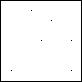
\includegraphics[width=0.3\textwidth]{gl_points}
  \caption{GL\_POINTS}
\end{figure}

\subsection{Primitivos de líneas}
\begin{itemize}
\item{GL\_LINES: Los vértices 0 y 1 se consideran una línea. Los vértices 2 y 3 se consideran una línea, y así progresivamente. Si el usuario especifica un número impar de vértices, el vértice extra es ignorado.}
\item{GL\_LINE\_STRIP: Los vértices adyacentes se consideran líneas. Entonces, si se pasan \textit{n} vértices, se producen \textit{n}-1 líneas. Si el usuario sólo pasa una línea se ignora el comando de dibujo.}
\item{GL\_LINE\_LOOP: Como el anterior excepto que el primer y último vértice también són usados como línea. Entonces, se producen \textit{n} líneas para \textit{n} vértices de entrada.}
\end{itemize}


\begin{figure} [h]
  \centering
  \captionsetup[subfigure]{justification=centering}
  \begin{subfigure}  {0.3\textwidth}
    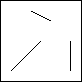
\includegraphics[width=\textwidth]{gl_lines}
    \caption{GL\_LINES}
  \end{subfigure}
  \begin{subfigure} {0.3\textwidth}
    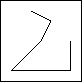
\includegraphics[width=\textwidth]{gl_line_strip}
    \caption{GL\_LINE\_STRIP}
  \end{subfigure}
  \begin{subfigure} {0.3\textwidth}
    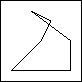
\includegraphics[width=\textwidth]{gl_line_loop}
    \caption{GL\_LINE\_LOOP}
  \end{subfigure}
  \caption{Primitivos de líneas}
\end{figure}

\restoregeometry


\newpage

\newgeometry{top=10mm, bottom=20mm}


\subsection{Primitivos triangulares}
Un triangulo es un primitivo formado por 3 vértices. Es la forma bidimensional con el menor número de vértices, así que los renderizadores normalmente están diseñados para rendierizar con ellos.
\begin{itemize}
\item{GL\_TRIANGLES: Los vértices 0, 1 y 2 forman un triángulo, Los vértices 3, 4 y 5 forman un triángulo, y así progresivamente.}
\item{GL\_TRIANGLE\_STRIP: Cada grupo de 3 vértices adyacentes forma un triángulo. Una lista de \textit{n} vértices forma \textit{n}-2 triángulos.}
\item{GL\_TRIANGLE\_FAN: El primer vértice siempre se mantiene fijo. De ahí en adelante, por cada grupo de dos vértices adyacentes se hará un triángulo con el primero. Una lista de \textit{n} vértices generará \textit{n}-2 triángulos.}
\end{itemize}

\begin{figure} [ht]
  \centering
  \captionsetup[subfigure]{justification=centering}
  \begin{subfigure} {0.3\textwidth}
    
\includegraphics[width=\textwidth]{gl_triangles}
    \caption{GL\_TRIANGLES}
  \end{subfigure}
  \begin{subfigure} {0.3\textwidth}
    
\includegraphics[width=\textwidth]{gl_triangle_strip}
    \caption{GL\_TRIANGLE\_STRIP}
  \end{subfigure}
  \begin{subfigure} {0.3\textwidth}
    
\includegraphics[width=\textwidth]{gl_triangle_fan}
    \caption{GL\_TRIANGLE\_FAN}
  \end{subfigure}
  \caption{Primitivos triangulares}
\end{figure}

\subsection{Primitivos \textit{quad}}
Un \textit{quad} es un primitivo cuadrilateral de cuatro vértices. Frecuentemente se tratan como un par de triangulos.
\begin{itemize}
\item{GL\_QUADS: Vértices 0-3 forman un quad, vértices 4-7 forman otro, y así progresivamente. El número de vértices en la lista debe de ser divisible por 4 para funcionar.}
\item{GL\_QUAD\_STRIP: De forma similar a GL\_TRIANGLE\_STRIP, un \textit{quad strip} utiliza los bordes adyacentes para formar el siguiente quad. En el caso de los quads, el tercer y cuarto vértice de un quad se utilizan para el siguiente \textit{quad}. De esta forma, los vértices 0-3 son un quad, 2-6 son otro quad y así progresivamente. Una lista de \textit{n} vértices generará \textit{n}-2 / 2 quads.}
\end{itemize}

\begin{figure} [h]
  \centering
  \captionsetup[subfigure]{justification=centering}
  \begin{subfigure}{0.3\textwidth} 
    
\includegraphics[width=\textwidth]{gl_quads} 
    \caption{GL\_QUADS}
  \end{subfigure}
  \begin{subfigure}{0.3\textwidth}
    
\includegraphics[width=\textwidth]{gl_quad_strip} 
    \caption{GL\_QUAD\_STRIP}
  \end{subfigure}
  \caption{Primitivos \textit{quad}}
\end{figure}

\restoregeometry

\section{Especificación de vértices usando la librería gráfica}
Es importante destacar que desde que se inicia la creación de un \textit{primitive} hasta que se termina \textbf{no} se puede utilizar una función de transformación.

\subsection{Inicio del \textit{primitve}}
Para iniciar la especificación de vértices hace falta llamar a la siguiente función
\begin{lstlisting}[language=C]
  glBegin(GLEnum mode)
\end{lstlisting}
Y como único argumento introducimos el tipo de primitivo (ver sección anterior).

\subsection{Pasar coordenadas de los vértices}
Existen diversas funciones para crear vertices, dependiendo de si quieren utilizar numeros flotantes o enteros, y si se quieren utilizar tres dimensiones o solo dos. Esas funciones son las siguientes.
\begin{lstlisting}[language=C]
  glVertex2f(GLfloat x, GLfloat y);
  glVertex2i(GLint x, GLint y);
  glVertex3f(GLfloat x, GLfloat y, GLfloat z);
  glVertex3i(GLint x, GLint y, GLint z);
\end{lstlisting}

\subsection{Pasar color de los vértices}
Cada vértice tiene un color con unos valores RGBA concretos, para asignarlos se usa una de las siguientes funciones.
\begin{lstlisting}[language=C]
  glColor3f(GLfloat red, GLfloat green, GLfloat blue);
  glColor3i(GLint red, GLint green, GLint blue);
  glColor4f(GLfloat red, GLfloat green, GLfloat blue, GLfloat alpha);
  glColor4i(GLint red, GLint green, GLint blue, GLfloat alpha);
\end{lstlisting}
De forma similar a pasar coordenadas a los vértices, existen diferentes funciones dependiendo de si se quiere pasar el valor \textit{alpha} o no, y dependiendo de el tipo de número.

Cabe destacar que con llamar a esta función una vez se aplica a todos los vértices especificados posteriormente (incluso si forman parte de otro primitivo) hasta que se vuelve a llamar la función con otro color.
\subsection{Finalizacion del \textit{primitive}}
Una vez que se han terminado de introducir los vertices, hace falta llamar a la siguiente funcion sin ningun argumento.
\begin{lstlisting}[language=C]
  glEnd();
\end{lstlisting}


%% Espacio de vista y transformación de la vista del modelo
\chapter{Espacio de vista y transformación de la vista del modelo}
\section{Matriz de transformación}
La matriz de transformación es aquella que se aplica a los diferentes vértices cuando son llamados y que acumula operaciones de \textbf{Translación}, \textbf{Rotación} y \textbf{Escalado}.
 \begin{figure}[ht]
   \centering
   \[
  \begin{bmatrix}
    1 && 0 && 0 && x\\
    0 && 1 && 0 && y\\
    0 && 0 && 1 && z\\
    0 && 0 && 0 && 1
  \end{bmatrix}
  \]
 \end{figure}
 \subsection{Operación: Reseteo}
Para restaurar la matriz a su estado original se hace uso de la función
\begin{lstlisting}[language=C]
  glLoadIdentity();
\end{lstlisting}
\subsection{Operación: Traslación}
Con la operación de Traslación se desplaza la matriz de transformación por un vector llamando a la función
\begin{lstlisting}[language=C]
  glTransformf(GLfloat x, GLfloat y, GLfloat z);
\end{lstlisting}
En los argumentos ponemos los valores del vector deseado.
\subsubsection{Operación matemática}
\(\overrightarrow{V}\) es el vector que hemos pasado como argumento, \(\mathbf{transf}\) es la matriz de transformación.
\begin{equation}
  \begin{bmatrix}
    1 && 0 && 0 && \overrightarrow{V}_x\\
    0 && 1 && 0 && \overrightarrow{V}_y\\
    0 && 0 && 1 && \overrightarrow{V}_z\\
    0 && 0 && 0 && 1
  \end{bmatrix}
  \cdot
  \begin{bmatrix}
    \mathbf{transf}_x\\\mathbf{transf}_y\\\mathbf{transf}_z\\1
  \end{bmatrix} =
  \begin{bmatrix}
    \mathbf{transf}_x'\\\mathbf{transf}_y'\\\mathbf{transf}_y'\\1
  \end{bmatrix}
\end{equation}


%% Espacio de clipping y transformación de proyección
\chapter{Espacio de clip y transformación de proyección}
En este paso los objetos son transformados del espacio de vista al espacio de clip utilizando la matriz \textbf{GL\_PROJECTION}. Esta matriz se utiliza para definir el frustum o tronco. Este frustum determina qué objetos o porciones de objetos serán recortados (\textit{clipped out}). También determina cómo se proyecta a la pantalla la escena 3D.

OpenGL proporciona dos funciones para la transformación de GL\_PROJECTION.

\begin{itemize}
\item{\textbf{glFrustum()}, para producir una proyección con perspectiva}
\item{\textbf{glOrtho()}, para producir una proyección ortográfica (paralela)}
\end{itemize}

Ambas funciones requieren 6 parámetros para especificar los 6 planos de corte; \textit{left}, \textit{right}, \textit{bottom}, \textit{top}, \textit{near} y \textit{far}.


También se puede utilizar \textbf{gluPerspective()}, que requiere de sólo 4 parámetros; el campo de vista vertical (FOV), la relación de aspecto de ancho a alto y las distancias a los planos de corte \textit{near} y \textit{far}. Es posible convertir la función gluPerspective() a glFrustum() con un código que será explicado en una sección posterior.

\section{Matriz de proyección (GL\_PROJECTION)}
Un monitor de ordenador es una superfície 2D. Una escena 3D renderizada por OpenGL tiene que ser proyectada a la pantalla del ordenador como una imagen 2D. La matriz GL\_PROJECTION es usada para esta transformación de proyección. Primero, la información de las coordenadas de vista es transformada a coordenadas de clip. Luego, estas coordenadas de clip son también transformadas a coorenadas normalizadas de dispositivo (NDC) dividiendo por el componente \textit{w} de las coordenadas de clip.

Por ello, tenemos que tener en cuenta que tanto el clipping (corte de frustum) como las transformaciones NDC están integradas en la matriz \textbf{GL\_PROJECTION}. Las siguientes secciones describen cómo construir la matriz de proyección utilizando 6 parámetros; \textit{left}, \textit{right}, \textit{bottom}, \textit{top}, \textit{near} y \textit{far}.

Nótese que el corte de frustum (clipping) se efectua en las coordenadas de clip, justo antes de dividir por $w_c$. Las coordenadas de clip, $x_c$, $y_c$ y $z_c$ se comprueban siendo comparadas con $w_c$. Si cualquiera de las coordenadas de clip es menor que $-w_c$, o más grande que $w_c$, entonces el vértice será descartado.
$ -w_c < x_c, y_c, z_c < wc $

Entonces, OpenGL rescunstruirá los filos del polígono donde ocurre el clipping.

\begin{figure} [h]
  \centering
  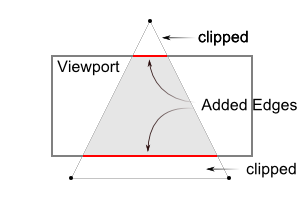
\includegraphics[width=0.3\textwidth]{gl_frustumclip}
  \caption{Un triangulo clipeado por el frustum}
\end{figure}

\section{Proyección de perspectiva}
En una proyección de perspectiva, un punto 3D en un en un frustum piramical truncado (coordenadas de vista) es mapeado a un cubo (NDC); el rango de la coordenada X desde [l, r] hasta [-1, 1], la coordenada Y desde [b, t] hasta [-1, 1] y la coordenada Z desde [n, f] hasta [-1, 1].

\begin{figure} [h]
  \centering
  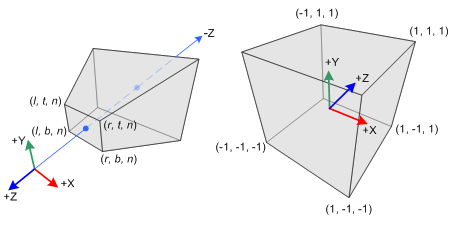
\includegraphics[width=0.6\textwidth]{gl_projectionmatrix01}
  \caption{Frustum de perspectiva y \textit{Normalized Device Coordinates} (NDC)}
\end{figure}


\newpage

Nótese que las coordenadas de vista están definidas por el sistema de coordenadas de la mano derecha, pero NDC utiliza el sistema de coordenadas de la mano izquierda. Por ello, la cámara en el origen está mirando a través del jee -Z en el espacio de vista, pero está mirando en el eje +Z en NDC. Puesto que \textbf{glFrustum()} sólo acepta valores positivos cómo distancias \textit{near} y \textit{far}, necesitamos negarlos durante la construcción de la matriz GL\_PROJECTION.

En OpenGL, un punto 3D en el espacio de vista es proyectado a el plano \textit{near} (plano de proyección). Los siguientes diagramas muestran como un punto $(x_e, y_e, z_e)$ en el espacio de vista está proyecatado a $(x_p, y_p, z_p)$ al plano \textit{near}.

\begin{figure} [h]
  \centering
  \captionsetup[subfigure]{justification=centering}
  \begin{subfigure}{0.3\textwidth} 
    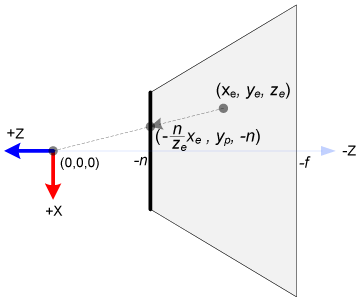
\includegraphics[width=\textwidth]{gl_projectionmatrix03} 
    \caption{Vista superior del Frustum}
  \end{subfigure}
  \begin{subfigure}{0.3\textwidth}
    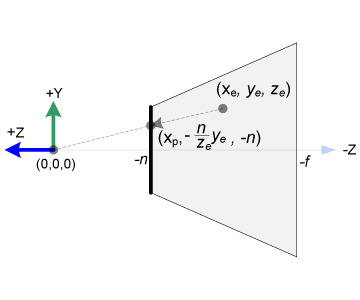
\includegraphics[width=\textwidth]{gl_projectionmatrix04} 
    \caption{Vista lateral del Frustum}
  \end{subfigure}
\end{figure}

Desde la vista superior del frustum, la coordenada X del espacio de vista, $x_e$ está mapeada a $x_p$, que es calculada utilizando la proporción de triangulos similares;
\begin{figure} [h]
  \centering
  \[
  \frac{x_p}{x_e} = \frac{-n}{z_e}
  x_p = \frac{-n \cdot x_e}{z_e} = \frac{n \cdot x_e}{-z_e}
  \]
\end{figure}

Desde la vista lateral del frustum, $y_p$ puede ser calculada con un método similar;

\begin{figure} [h]
  \centering
  \[ \frac{y_p}{y_e} = \frac{-n}{z_e}
  y_p = \frac{-n \cdot y_e}{z_e} = \frac{n \cdot y_e}{-z_e} \]
\end{figure}

\newpage

Nótese que tanto $x_p$ como $y_p$ dependen de $z_e$; son inversamente proporcionales a $-z_e$. En otras palabras, ambas están divididas por $-z_e$. Esta es la primera pista para la construcción de la matriz GL\_PROJECTION. Después de que las coordenadas sean transformadas multiplicando la matriz GL\_PROJECTION, las coordenadas siguien siendo coordenadas homogéneas. Se vuelven finalmente \textit{Normalized Device Coordinates} (NDC) cuando se dividen por el componente \textit{w} de las coordenadas de clip.

\begin{figure} [h]
  \centering
  \[
  \begin{pmatrix}
    x_{clip} \\ y_{clip} \\ z_{clip} \\ w_{clip}
  \end{pmatrix}
  =
  M_{projection} \cdot
  \begin{pmatrix}
    x_{vista} \\ y_{vista} \\ z_{vista} \\ w_{vista}
  \end{pmatrix} ,
  \begin{pmatrix}
    x_{ndc} \\ y_{ndc} \\ z_{ndc}
  \end{pmatrix}
  =
  \begin{pmatrix}
    x_{ndc}/w_{clip} \\ y_{ndc}/w_{clip} \\ z_{ndc}/w_{clip}
  \end{pmatrix}
  \]
\end{figure}


Entonces, podemos definir el componente \textit{w} de las coordenadas de clip como $-z_e$. Y la cuarta fila de la matriz GL\_PROJECTION se vuelve (0, 0, -1, 0).


\begin{figure} [h]
  \centering
  \[
  \begin{pmatrix}
    x_{c} \\ y_{c} \\ z_{c} \\ w_{c}
  \end{pmatrix}
  =
  M_{projection} \cdot
  \begin{pmatrix}
    \cdot && \cdot && \cdot && \cdot \\
    \cdot && \cdot && \cdot && \cdot \\
    \cdot && \cdot && \cdot && \cdot \\
        0 &&     0 &&    -1 &&     0
  \end{pmatrix} \cdot
  \begin{pmatrix}
    x_{e} \\ y_{e} \\ z_{e} \\ w_{e}
  \end{pmatrix}
  ,  \therefore w_c = -z_e
  \]
\end{figure}


%% Espacio NDC y división de perspectiva
\newgeometry {margin=4cm, hmargin= 2cm}
\chapter{Espacio de la pantalla}
\section{Conversión a coordenadas de la pantalla}
Una vez se tienen las coordenadas de los puntos entre las coordenadas (-1, -1) y (1, 1) se busca encontrar la coordenada correspondiente en la pantalla.
\begin{itemize}
  \item{\(x_d\) es la coordenada en la pantalla}
  \item{\(x_s\) es la coordenada real normalizada}  
  \item{\(x_m\) es la coordenada donde comienza la superficie en la que queremos dibujar}
  \item{\(x_M\) es la coordenada donde termina la superficie en la que queremos dibujar}  
  \item{\(\Delta x = x_M - x_m\)}
\end{itemize}
\begin{equation*}
  \frac{x_s-(-1)}{1-(-1)} = \frac{x_d - x_m}{\Delta x}
\end{equation*}
Si aislamos \(x_d\) obtenemos la siguiente ecuación:
\begin{equation*}
  x_d = \frac{\Delta x \cdot x_s}{2}+\frac{\Delta x}{2}+x_m
\end{equation*}
En el caso de la coordenada \(y\) funciona igual excepto que cambiamos el sentido así que tiene una pequeña variación.
\begin{equation*}
  y_d = \frac{-(\Delta y) \cdot y_s}{2}+\frac{\Delta y}{2}+y_m
\end{equation*}
Y en forma de matriz, la operación quedaría así.

\begin{equation*}
  \begin{bmatrix}
     \frac{\Delta x}{2} && 0 && \frac{\Delta x}{2} + x_m\\
     0 && - \frac{\Delta y}{2} && \frac{\Delta y}{2} + y_m \\
     0 && 0 && 1
  \end{bmatrix}
  \cdot
  \begin{bmatrix}
    x_s\\
    y_s\\
    1
  \end{bmatrix}
  =
  \begin{bmatrix}
    x_d\\
    y_d\\
    1
  \end{bmatrix}
\end{equation*}
\restoregeometry

\section{Funcionamiento de SDL2}
Uno de los objetivos de este Treball de Recerca era utilizar una librería que permitiera compilar y ejecutar el programa en los principales Sistemas Operativos y entornos de desarrollo.

SDL2 es una librería de desarrollo multi-plataforma, que proporciona acceso de nivel bajo al audio, teclado, ratón y hardware gráfico utilizando OpenGL.

Es por eso que ha sido de vital importancia, ya que nos ha permitido simular el funcionamiento de OpenGL sin necesidad de tener que recrear partes más técnicas y complejas que no tenían relevancia en este proyecto.

En general, ha permitido crear, de forma sencilla, un entorno sobre el que aplicar la librería gráfica (tanto la de OpenGL como la nuestra propia).

\subsection{Cómo lo he usado}
SDL2 ofrece dos métodos para la gestión de gráficos, en uno se utiliza OpenGL directamente, se llama a funciones de OpenGL y se trabaja como lo haría OpenGL.

Sin embargo, también existe un método en el que OpenGL se limita a funcionar como comunicador a la tarjeta gráfica.

Este doble funcionamiento ha sido vital, pues ha permitido crear dos versiones del programa. En la primera, OpenGL se usa plenamente. En la segunda, todas las funciones de OpenGL se han mimetizado para intentar comprender cuál es su funcionamiento. Esto ha permitido crear comparaciones entre las dos versiones.


Ahora se explicarán algunas de las funciones de SDL2 que se han ido usando a lo largo del código y que hace falta definir. Para explorar estas funciones y SDL2 en general, existe un sitio oficial\footnote{https://wiki.libsdl.org} que funciona a modo de documentación.


\subsection{Funciones importantes de SDL2 - OpenGL}
Estas son las funciones relevantes para la versión del programa que utiliza plenamente OpenGL.


\subsubsection{Inicialización de SDL2}
Para iniciar un entorno de SDL2 se llama a la siguiente función:
\begin{lstlisting}[language=C]
  int SDL_Init(Uint32 flags)
\end{lstlisting}
Como parámetro, se pueden añadir flags de inicialización como por ejemplo
\textit{SDL\_INIT\_VIDEO}, para inicializar el vídeo.

\subsubsection{Creación de ventana}
Para crear una ventana se llama a esta función:
\begin{lstlisting}[language=C]
  SDL_Window* SDL_CreateWindow(const char* title,
                              int x, int y, int w, int h, 
                              Uint32 flags)
\end{lstlisting}
Donde los parámetros son el título, las coordenadas \textit{x} y \textit{y} iniciales, w y h son la anchura y la altura, respectivamente y además se puede añadir alguna opción en flag, en este caso, es necesario añadir SDL\_WINDOW\_OPENGL para indicar que esta ventana se destinará a OpenGL.

\subsubsection{Creación de contexto}
En la anterior función se creó la ventana, pero ahora hace falta crear el entorno (contexto) de renderización de OpenGL.
\begin{lstlisting}[language=C]
  SDL_GLContext SDL_GL_CreateContext(SDL_Window* window)
\end{lstlisting}
El único parámetro es la ventana previamente creada en la cuál queremos crear el contexto de renderización.

\subsubsection{Actualización de la ventana}
Puesto a que se está utilizando OpenGL será necesario llamar a
\begin{lstlisting}[language=C]
  void SDL_GL_SwapWindow(SDL_Window* window)
\end{lstlisting}
Con esta función se actualizará la ventana actual con el búfer\footnote{Espacio de memoria en el que se almacenan los datos de forma temporal} de OpenGL.

\subsubsection{Finalización de SDL2}
Una vez que se desea terminar con la ejecución del programa, hay que terminar antes el entorno de SDL2 con las siguientes funciones.
\begin{lstlisting}[language=C]
  void SDL_DestroyWindow(SDL_Window* window)
\end{lstlisting}
El único parámetro es la ventana que se desea finalizar.
\begin{lstlisting}[language=C]
  void SDL_Quit()
\end{lstlisting}

Para la demás funcionalidad, hay que referirse a OpenGL.

\subsection{Funciones importantes de SDL2 - sin OpenGL}
\subsubsection{Inicialización de SDL2}
Para iniciar un entorno de SDL2 se llama a la siguiente función:
\begin{lstlisting}[language=C]
  int SDL_Init(Uint32 flags)
\end{lstlisting}
Como parámetro, se pueden aladir flags de inicialización como por ejemplo \textit{SDL\_INIT\_VIDEO}, para inicializar el vídeo.

\subsubsection{Creación de ventana}
Para crear una ventana se llama a esta función:
\begin{lstlisting}[language=C]
  SDL_Window* SDL_CreateWindow(const char* title,
                               int x, int y, int w, int h,
                               Uint32 flags)
\end{lstlisting}
Donde los parámetros son el título, las coordenadas \textit{x} y \textit{y} iniciales, w y h son la anchura y la altura, respectivamente y además se puede añadir alguna opción en flag.

\subsubsection{Creación de renderizador}
Puesto a que no estamos utilizando OpenGL de forma directa, es necesario crear un Renderer que gestione lo que SDL tiene que dibujar.
\begin{lstlisting}
  SDL_Renderer* SDL_CreateRenderer(SDL_Window* window,
                int index, Uint32 flags)
\end{lstlisting}
El primer parámetro es la ventana en la que se desea dibujar, la segunda es el índice del dispositivo de renderización (medio que se quiere utilizar para los gráficos) y finalmente una flag que indique el tipo de renderización a usar.


\subsubsection{Cambio de color}
En lugar lugar de escoger el color cada vez que se dibuja algo, SDL2 guarda el último color seleccionado y es el que utiliza hasta que se llama a la siguiente función.
\begin{lstlisting}[language=C]
  void SDL_SetRenderDrawColor(SDL_Renderer* renderer,
       int8 r, Uint8 g, Uint8 b, Uint a)
\end{lstlisting}
El primer parámetro es el contexto de renderización que se está utilizando, y los siguientes son los valores RGBA, que definen el color y oscilan del 0 al 255 cada uno.

\subsubsection{Dibujo de puntos}
Para dibujar un punto, simplemente hay que usar la siguiente función.
\begin{lstlisting}[language=C]
  int SDL_RenderDrawPoint(SDL_Renderer* renderer,
                         int x, int y)
  
\end{lstlisting}
El primer parámetro es el contexto usado actualmente. Los valores \textit{x} y \textit{y} corresponden a la coordenada de la pantalla en la que se desea dibujar un punto.

\subsubsection{Dibujo de líneas}
Para dibujar una línea, funciona de forma similar a un punto, pero con una coordenada adicional (la final).
\begin{lstlisting}[language=C]
  int SDL_RenderDrawLine(SDL_Renderer* renderer,
                        int x1, int y1,
                        int x2, int y2)
\end{lstlisting}
El primer parámetro es el contexto de renderización que se está utilizando, \textit{x1} y \textit{y1} corresponden a la coordenada origen de la línea y \textit{x2} y \textit{y2} corresponden a la coordenada final de la línea.


En caso de de no estar utilizando OpenGL directamente, se puede llamar a
\begin{lstlisting}[language=C]
  void SDL_RenderPresent(SDL_Renderer* renderer)
\end{lstlisting}
El único parámetro es el renderer utilizado actualmente.

\subsubsection{Actualización de la ventana}
Una vez se hayan aplicado todas las operaciones que se deseen, se ha de llamar a la siguiente función para mostrarlo.
\begin{lstlisting}[language=C]
  void SDL_RenderPresent(SDL_Renderer* renderer)
\end{lstlisting}
El único parámetro es el renderizador que se quiere actualizar.
\newpage

\subsubsection{Finalización de SDL2}
La forma de finalizar SDL2 cuando no se ha usado directamente OpenGL es un poco más compleja.
Primero hace falta destruir el renderer que se ha usado.
\begin{lstlisting}[language=C]
  void SDL_DestroyRenderer(SDL_Renderer* renderer)
\end{lstlisting}
Posteriormente, se destruye la ventana.
\begin{lstlisting}[language=C]
  void SDL_DestroyWindow(SDL_Window* window)
\end{lstlsiting}

Finalmente, se cierra el entorno de SDL.
\begin{lstlisting}[language=C]
  void SDL_Quit()
\end{lstlisting}

\section{Estructura del código}

El código se estructura en dos tipos de archivos, unos compatibles con
OpenGL y con nuestra adaptación de la librería y otros que son los que
sustuyen parcialmente la funcionalidad de OpenGL. 

\textbf{Archivos genéricos}
\begin{itemize}
	\item [\textbf{Examples}] Contiene diferentes ejemplos de escenas que incluyen objetos definidos en el archivo \textit{Objects} con la finalidad de comprobar el funcionamiento correcto de la implementación.
	\item [\textbf{Init}] Inicializa la comunicación gráfica entre software y hardware, es decir, entre el programa y la tarjeta gráfica,  mediante la librería SDL2.
	\item [\textbf{main}] Es donde comienza y acaba el programa, haciendo las llamadas necesarias a las diferentes partes del programa para su continua ejecución.
	\item [\textbf{Objects}] Instucciones para crear objetos gráficos individuales, que agrupados formarán los ejemplos.
	\item [\textbf{Renderer}] Es donde se encuentra el bucle de renderización de la escena, además de contener dos funciones de utilidad gráfica para simplificar la visualización en perspectiva, deprecadas en las últimas versiones de OpenGL.
\end{itemize}

\newpage

\textbf{Archivos específicos}
\begin{itemize}
	\item [\textbf{Execute}] Es el archivo que contiene una función llamada desde la función inicial main() en cada bucle de renderización. Se encarga de dos cosas principalmente, la primera es inicializar las variables que se necesitan para los cálculo gráficos y la segunda es la manipulación y gestión de las estructuras de memoria gráfica en cada ciclo.
	\item [\textbf{List}] Es una lista que contiene todas las intrucciones que se tienen que ejecutar en cada ciclo del programa.
	\item [\textbf{Matrix}] Se realizan algunas operaciones con matrices necesarias, como es: multiplicar dos matrices, inversa de una matriz, matriz por un vector, normalizar un vector, ...
	\item [\textbf{Model}] Contiene las definiciones de las variables del modelo. Matrices de rotación, translación y escalado, matriz que guarda el último movimiento realizado y los elementos mínimos de funcionamiento del programa, los nodos.
	\item [\textbf{Node}] Manipula los elementos mínimos del programa, los nodos. Aquí se crean y se destruyen. También es donde se enlazan con el siguiente.
	\item [\textbf{Scanner}] En este archivo se interpretan las instrucciones y se va creando una lista de nodos a ejecutar en el ciclo actual, guardándose todas en un pila.
	\item [\textbf{Stack}] Manipula las pilas, es decir, las crea, las destruye y las enlaza con la siguiente. Estas pilas serán recorridas y ejecutadas para crear la escena.
	\item [\textbf{TRGL}] Encapsula funciones análogas a las OpenGL, de manera que sea posible utilizar la librería OpenGL o el propio motor gráfico con sólo cambiar un parámetro del make (la compilación).
\end{itemize}



\begin{figure}[h]
 \centering
 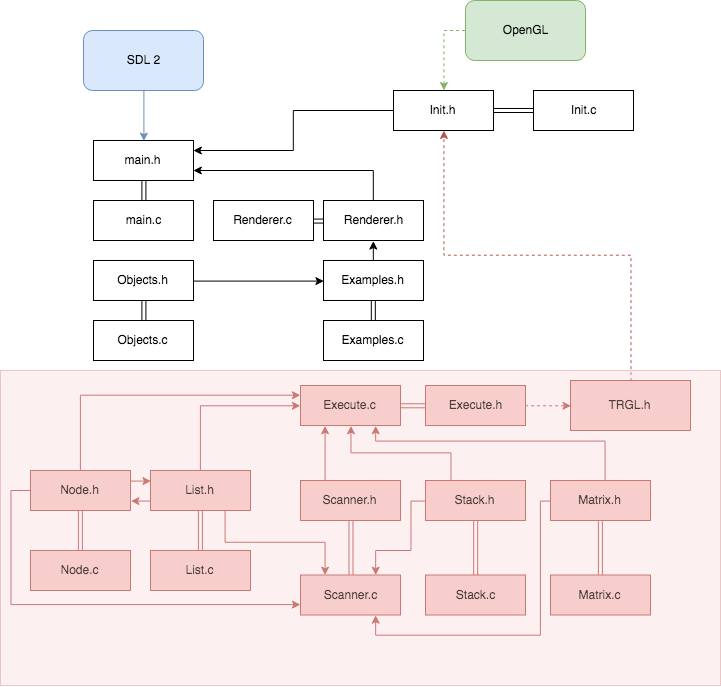
\includegraphics[width=\textwidth]{diagrama}
\end{figure}


%% Espacio de la pantalla y escalado y translación
\newgeometry{margin=3cm, hmargin=2cm}
\chapter{Valoración general y conclusión}
\section{Procesos por los que pasó el Treball de Recerca}
Inicialmente el objetivo del Treball de Recerca era el de crear una escena tridimiensional interactiva en la que se mostrase alguna figura. Tras unas pocas semanas, nos dimos cuenta de que hoy en día existen muchas herramientas para realizar esto, pero nos daba la sensación de que no se comprendía muy bien cómo funcionaba, y por lo tanto no era honesto simplemente utilizar esas herramientas, duramente se podría extraer una conclusión.

Por ello decidimos ir un paso más allá e intentar crear nosotros mismos esas herramientas, es decir, crear una librería gráfica con nuestras propias funciones que asimilaran lo que hacían las librerías gráficas populares. Sin embargo hicimos un poco de trampa, pues es increíblemente difícil crear un software que se comunique propiamente con una tarjeta gráfica moderna (hoy en día vienen bloqueadas y se requiere contactar con el fabricante para tener el permiso). Además de la dificultad del proceso, es importante recordar que el enfoque que pretendíamos dar a este trabajo era matemático y no técnico o tecnológico, por lo que entrar en detalle sobre el funcionamiento de una tarjeta gráfica moderna se escapaba de las intenciones originales y no es representativo de una situación moderna en un equipo de desarrollo de Software.

Por lo tanto, nuestra \textit{librería gráfica} utilizaba OpenGL en el fondo, pero éste sólo se dedicaba a comunicarse con la tarjeta, y la manipulación los vértices, el cálculo operaciones y la decisión de qué se muestra en la pantalla quedaron relegados a nuestra librería gráfica.

Aunque parezca que el trabajo se ha simplificado mucho, aún seguía siendo una tarea mucho más laboriosa que el acercamiento original. Esta nueva dirección nos permite atajar algo tan complejo como el mundo de los motores gráficos con preguntas relativamente básicas cómo:
\begin{itemize}
\item{¿Cómo se hace una línea?}
\item{¿Qué operaciones se tienen que aplicar para pasar de coordenadas imaginarias las coordenadas concretas de una ventana?}
\item{¿Cómo funciona la ocultación de caras?}
\item{¿Cómo se calcula la rotación de un punto en tres dimensiones?}
\end{itemize}

Y estas son sólo unas pocas de las docenas que han surgido a lo largo del Treball de Recerca y se han ido respondido de forma bastante satisfactoria. Claro está, los recursos son los que hay y han habido cuestiones que han sido más difíciles y prácticamente imposibles de resolver, pero que al menos han surgido en primer momento.


\newpage
Finalmente, coincidiendo con la aproximación de la fecha de entrega del documento redactado, tocó el momento de trazar la línea y intentar pasar a centarnos en cómo enfocar la defensa del Treball de Recerca. Para esta, al no ser importante el conocimiento adquirido, usaremos herramientas que nos permitan comunicar y explicar el trabajo de una forma más directa y comprensible.

\section{Revisión de la hipótesis}
La hipótesis inicial era la siguiente:

\textit{Los equipos de desarrollo de software deberían de aspirar a ser ellos mismos quienes crean las herramientas que utilizarán para crear el software en sí. En caso de que esta sea una decisión no rentable, su máxima prioridad debería de ser entender cómo funcionan las herramientas que utilizarán.}

Aunque quizás puede parecer que este trabajo sea más una compilación de cómo funciona una librería gráfica desde un punto matemático más que un intento de comprobar esta hipótesis, yo era plenamente consciente de esto a la hora de formularla. Pensé que ser capaz de crear algo similar a una librería gráfica debería de proporcionarme el conocimiento para determinar si alguien con un cierto conocimiento previo sobre ordenadores y programación necesita adentrarse plenamente en los fundamientos de un motor gráfico para poder llegar a usarlo correctamente.

La evidencia de que este parece ser el caso se encuentra en los commits\footnote{actualización que hace un programador del código de un repositorio} que han ido ocurriendo a lo largo de la elaboración del código que acompaña este treball de recerca. Es muy fácil apreciar que en cuestión de semanas se pasa de utilizar operaciones ineficientes, guardar información inútil y en general hacer un mal uso de las funciones creadas a utilizar matrices y punteros para optimizar la velocidad y incluso aportar un cierto nivel de modularidad.

Por lo tanto, me parece justo establecer que el mundo de los gráficos computables requiere que el programador sea altamente consciente del funcionamiento interno del mismo para poder hacer un uso óptimo.

La prueba definitiva de que mi hipótesis es verdad se halla en la evolución de OpenGL como librería gráfica. En las versiones originales de OpenGL (1 y 2), la misma librería gráfica, además de gestionar la comunicación con la tarjeta gráfica, hace todos los cálcuos y gestiona los vértices. Sin embargo, en la versión más reciente, OpenGL ha quedado completamente relegado a comunicación directa con la tarjeta gráfica, y todas las funciones de más (justamente las mismas que hemos creado nosotros en nuestra librería gráfica) han creado deprecadas y ahora es tarea del equipo de desarrollo que usa OpenGL crear las suyas propias, pensadas para funcionar de forma óptima en ese proyecto, pues un motor, o incluso librería, con uso general, parece ser cada vez más inviable.

\section{Opinión personal}
Estoy muy satisfecho con el resultado de este Treball de Recerca. Aunque he intentado dejar este documento lo más teórico posible, la mayoría de horas se han invertido en progaramar el motor gráfico utilizando la teoría que se ha expuesto. Espero poder continuar investigando sobre el complejo mundo de los motores gráficos más adelante, pero ciertamente este primer trabajo ha servido para tener una (limitada, pero no negligible) idea de cómo funciona la investigación.

\section{Bibliografía}
Diversos de estos recursos se han ido usando simultáneamente a lo largo del Treball de Recerca
\begin{itemize}
\item{Wiki de SDL2 \\ \url{https://wiki.libsdl.org}}
\item{Página web de Song Ho Ahn sobre OpenGL \\\url{https://www.songho.ca/opengl/index.html}}
\item{Página web de referencia oficial sobre OpenGL de Khronos \\\url{https://www.khronos.org/registry/OpenGL-Refpages/}}
\item{Wiki de \LaTeX \\ \url{https://en.wikibooks.org/wiki/LaTeX}}
\item{El repositorio del Treball de Recerca creado por mi, crucial para la comprensión del mismo\\
  \url{https://github.com/gorostuck/treball-recerca}}
\end{itemize}


\end{document}

